%%%%%%%%%%%%%%%%%%%%%%%%%%%%%%%%%%%%%%%%%%%%%%%%%%%%%%%%%%%%%%%%%%%%%%%%%%%%%
%	E-Yantra, IIT-Bombay

%	Document Author: Saurav Shandilya
%	Date: 16-August,2012

%%%%%%%%%%%%%%%%%%%%%%%%%%%%%%%%%%%%%%%%%%%%%%%%%%%%%%%%%%%%%%%%%%%%%%%%%%%%%

\documentclass[10pt,red]{beamer} 
% change the alerted colour to blue
\setbeamercolor{alerted text}{fg=blue}

\usetheme{berlin}
%\usetheme{warsaw}

%\usecolortheme{rose}
% theme split
\usepackage{beamerthemesplit}

% theme shadow
%\usepackage{beamerthemeshadow}

% For including figures
\usepackage{graphicx}

% logo
\logo{
\includegraphics[height=0.8cm]{iitblogo.pdf}}


% sf family, bold font
\sffamily \bfseries
% Beginning of title page
\title
% content inside [] appears at bottom of all page. content inside {} appears on first page as title. double backslash means line change 
[
	Firebird LPC2148 Robotics Research Platform	% bottom
	\hspace{0.5cm}
	\insertframenumber/\inserttotalframenumber
]
{
	Introduction to Firebird-V \\ Robotics Research Platform
}

\author
[
	www.e-yantra.org
]
{
	e-Yantra Team \\[20pt]
  Embedded Real-Time Systems Lab\\
  Indian Institute of Technology-Bombay \\
}
\date
{
IIT Bombay \\ 29 June 2015
}
 
 
\begin{document}  

%Slide-1 for title page
\begin{frame}
   \titlepage
\end{frame}

%Slide-2 Content & Agenda for Talk 
\section*{outline}
\begin{frame}[shrink = 8]
	\frametitle{Agenda for Discussion}
	\tableofcontents
\end{frame}
 
% Start of Section-1: Introduction to Robotics & Firebird
\section{Introduction to Robotics}
\subsection{Major Components of a Robot}
%Slide-3 Major Building Blocks of Robot 
\begin{frame}
	\frametitle{Major Building Blocks of Robot} 
	What are the Major Components needed for Designing a Robot? \pause \\[5pt]
	\begin{enumerate}
	\item <+-|alert@+> Sensors: For Sensing the environments \\[5pt]
	\item <+-|alert@+> Actuators: For Movement of robots and its parts \\[5pt]
	\item <+-|alert@+> Control: Controller/Processor as brain of Robot \\[5pt]
	\item <+-|alert@+> Intelligence: User Written Command to perform desired set of action \\[5pt]    
	\item <+-|alert@+> Power: A necessity for making a system work \\[5pt]
	\item <+-|alert@+> Communication: Robot can talk to another robot/PC \\[5pt]
	\end{enumerate}
\end{frame}

%\subsection{Definition of a Robot}
%Slide-4 Definition of a Robot
%\begin{frame}
%	\frametitle{Definition Of Robotics}
%\end{frame}

% End of Section-1: Introduction to Robotics & Firebird

% Start of Section-2: Introduction to Firebird
\section{Introduction to FireBird Platform}
%Slide-5 Various Configuration of FB
\begin{frame}
	\frametitle{Flavors of Firebird Robots} \pause
	\begin{enumerate}
		\item<+-|alert@+> Configuration-1: \\ Master: P89v51RD2\qquad \hspace{7pt} Slave: ATmega 2560  
		\item<+-|alert@+> Configuration-2: \\ Master: ATmega 2560\qquad Slave: ATmega 8 		
		\item<+-|alert@+> Configuration-3: \\ Master: LPC 2148\qquad \hspace{12pt} Slave: 2 x ATmega 8 
	\end{enumerate}
\end{frame}
%******** Start of subsection-1*************
\subsection{Firebird V 8051 Platform}
%Slide-6 8051
\begin{frame}
	\frametitle{Firebird V P89v51RD2 Platform} \pause
		\begin{minipage}[c]{0.4\textwidth}
			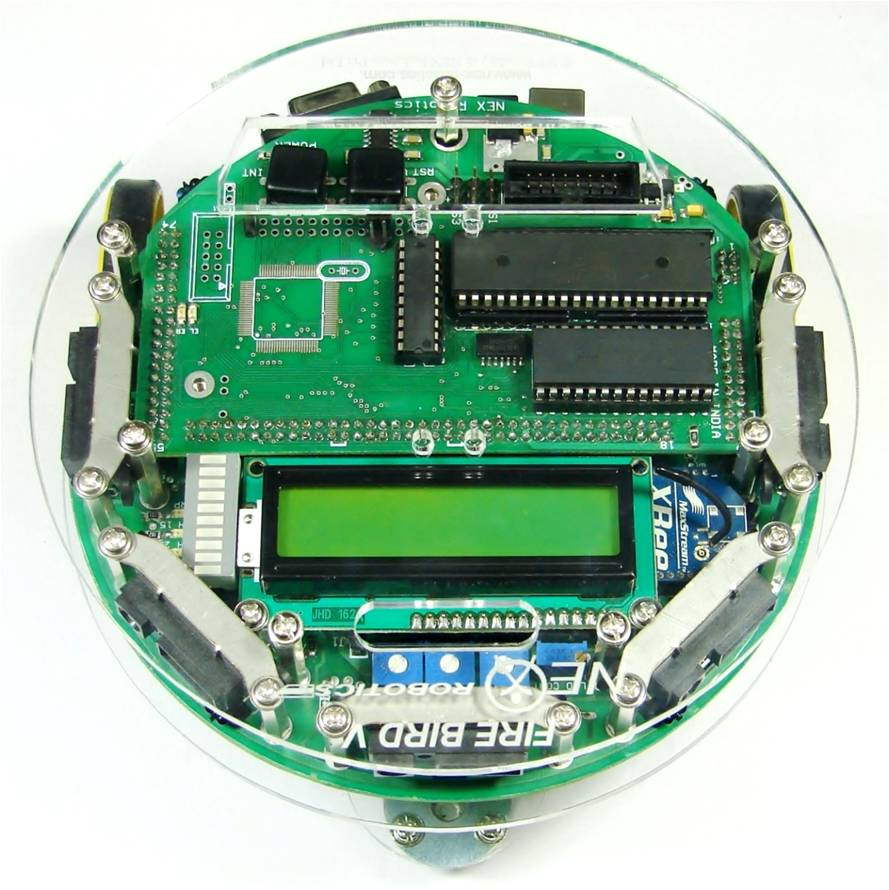
\includegraphics[width=\linewidth]{fb_v_8051}
		\end{minipage}
	\pause
	\hfill
		\begin{minipage}[c]{0.5\textwidth}
			\begin{enumerate}
				\item <+-|alert@+> This Platform has 8051 architecture based adaptor board.
				\item <+-|alert@+> Microcontroller used is Philips manufactured P89v51RD2 as master.
			\end{enumerate}
		\end{minipage}   
\end{frame}
%******** End of subsection-1*************

%******** Start of subsection-2*************
\subsection{Firebird V AVR Platform}
%Slide-7 AVR
\begin{frame}
	\frametitle{Firebird V ATmega2560 Platform} \pause
		\begin{minipage}[c]{0.4\textwidth}
			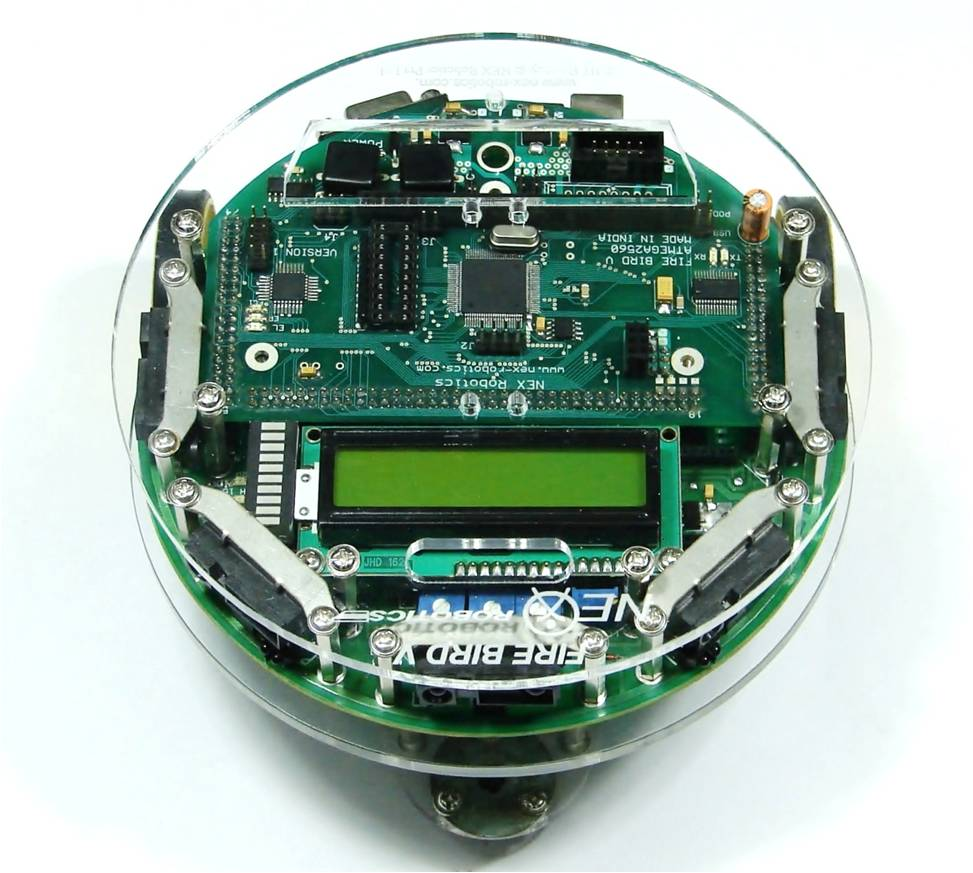
\includegraphics[width=\linewidth]{fb_v_avr}
		\end{minipage}
	\pause
	\hfill
		\begin{minipage}[c]{0.5\textwidth}
			\begin{enumerate}
				\item <+-|alert@+> This Platform has AVR architecture based adaptor board.
				\item <+-|alert@+> Microcontroller used is Atmel manufactured ATmega2560 as master.
			\end{enumerate}
		\end{minipage}   
\end{frame}

%******** End of subsection-2***************

%******** Start of subsection-3*************
\subsection{Firebird V ARM Platform}
%Slide-8 ARM-7
\begin{frame}
	\frametitle{Firebird V LPC 2148 Platform} \pause
		\begin{minipage}[c]{0.4\textwidth}
			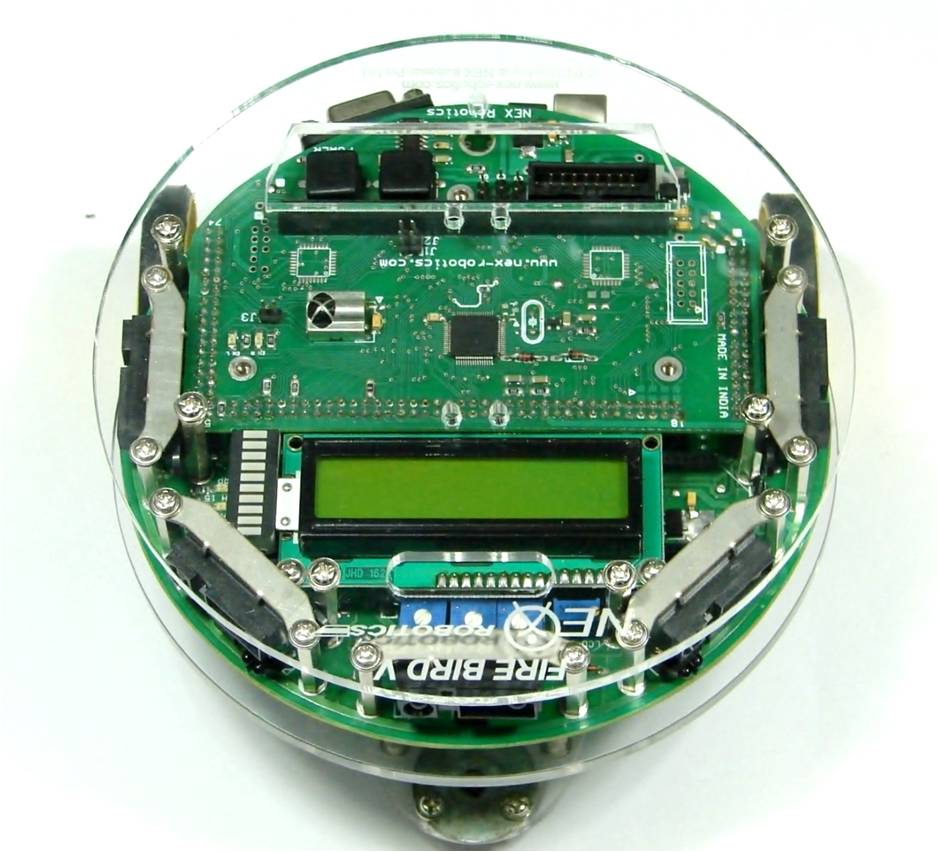
\includegraphics[width=\linewidth]{fb_v_arm}
		\end{minipage}
	\pause
	\hfill
		\begin{minipage}[c]{0.5\textwidth}
			\begin{enumerate}
				\item <+-|alert@+> This Platform has ARM-7 architecture based adaptor board.
				\item <+-|alert@+> Microcontroller used is Philips manufactured LPC2148 as master.
			\end{enumerate}
		\end{minipage}   
\end{frame}

%******** End of subsection-3***************

% End of Section-2: Introduction to Firebird

% Start of Section-3: Firebird V LPC2148 
\section{Introduction to FireBird LPC2148 Platform}
%******** Start of subsection-1*************
\subsection{Major Components of a Robot}
%Slide-9 Major components
\begin{frame}
	\frametitle{Major Building Blocks of Robot} 
	The Major Components needed for Designing a Robot  
	\begin{itemize}
		\item <1-> Sensors: For Sensing the environments \\[5pt]
		\item <1-> Actuators: For Movement of robots and its parts \\[5pt]
		\item <1-> Control: Controller/Processor as brain of Robot \\[5pt]
		\item <1-> Intelligence: User Written Command to perform desired set of action \\[5pt]    
		\item <1-> Power: A necessity for making a system work \\[5pt]
		\item <1-> Communication: Robot can talk to another robot/PC \\[5pt]
	\end{itemize}
\end{frame}
%******** End of subsection-1*************

%******** Start of subsection-2 (Senosr)*************
\subsection{Sensors}
%Slide-10 IR Sharp
\begin{frame}
	\frametitle{Sensors on Firebird V Platform} 
	1. Sharp IR Range Sensors	\pause
		\vfill
		\begin{minipage}[c]{0.5\textwidth}
			\begin{enumerate}
				\item <+-|alert@+> Transmitter: IR ray \qquad Receiver: CCD Array \\[10pt]
				\item <+-|alert@+> Count on Firebird: 05
			\end{enumerate}
		\end{minipage}
		%\pause
		\hfill
		\begin{minipage}[c]{0.4\textwidth}
			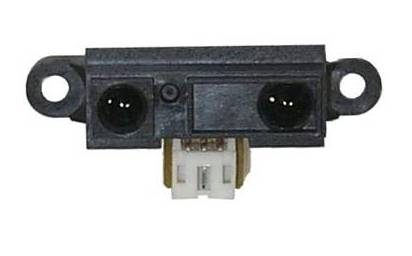
\includegraphics[width=0.8\linewidth]{ir_sharp}
		\vfill
			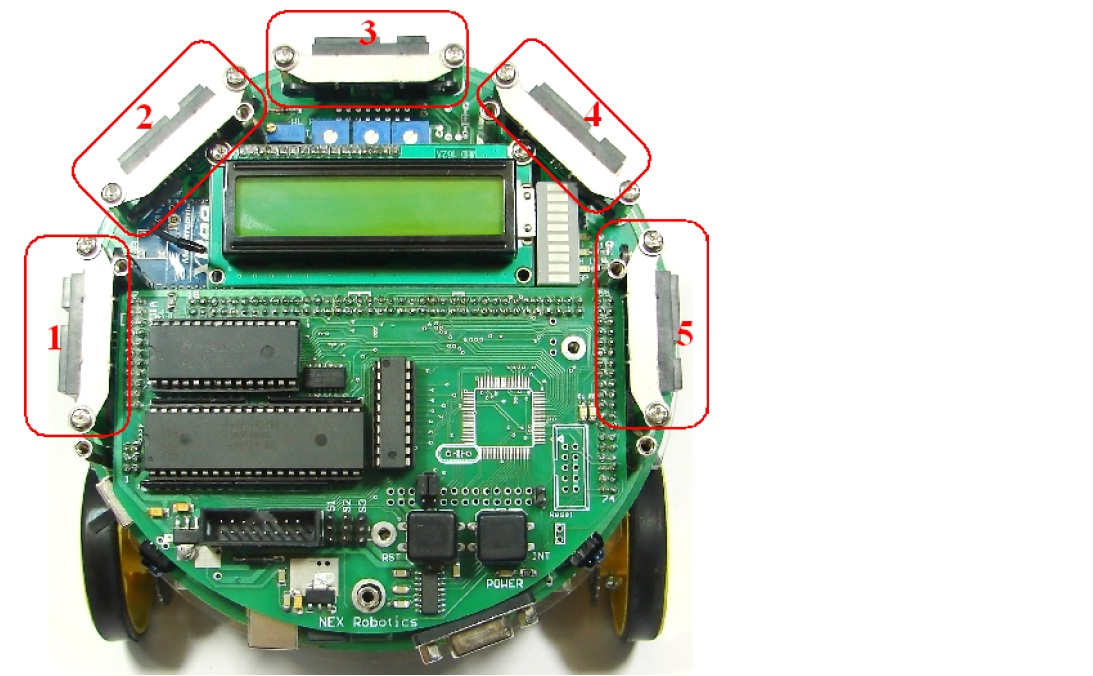
\includegraphics[width=\linewidth]{sharp_on_fb}
		\end{minipage}	
\end{frame}

%Slide-11 IR Proximity
\begin{frame}
	\frametitle{Sensors on Firebird V Platform (cont.)} 
	2. IR Proximity Sensors	\pause
		\vfill
		\begin{minipage}[c]{0.5\textwidth}
			\begin{enumerate}
				\item <+-|alert@+> Transmitter: IR ray \qquad Receiver: Phototransistor \\[10pt]
				\item <+-|alert@+> Count on Firebird: 08
			\end{enumerate}
		\end{minipage}
	%	\pause
		\hfill
		\begin{minipage}[c]{0.4\textwidth}
			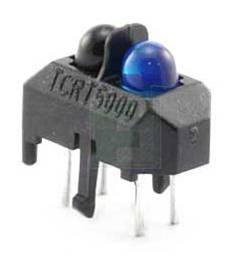
\includegraphics[width=0.4\linewidth]{ir_proximity}
		\vfill
			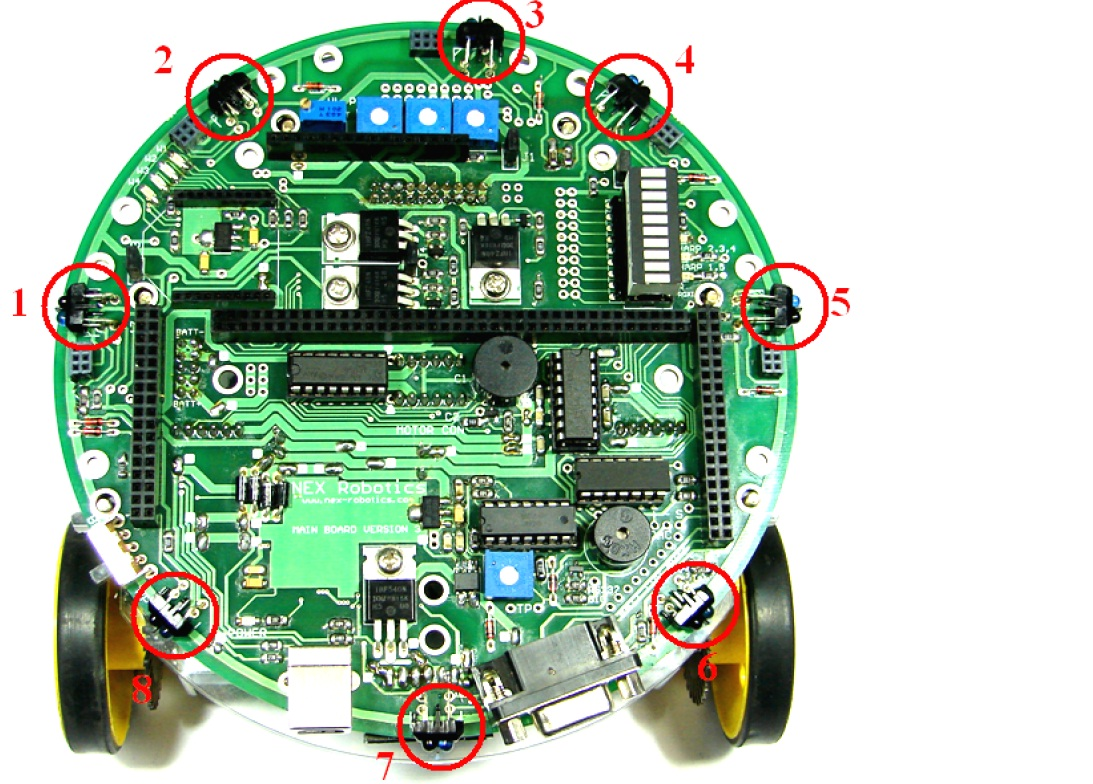
\includegraphics[width=0.8\linewidth]{proximity_on_fb}
		\end{minipage}
\end{frame}

%Slide-12 White Line
\begin{frame}
	\frametitle{Sensors on Firebird V Platform (cont.)} 
	3. White Line Sensor	\pause
		\vfill
		\begin{minipage}[c]{0.5\textwidth}
			\begin{enumerate}
				\item <+-|alert@+> Transmitter: Red LED \qquad Receiver: PhotoTransistor \\[10pt]
				\item <+-|alert@+> Count on Firebird: 01
			\end{enumerate}
		\end{minipage}
		%\pause
		\hfill
		\begin{minipage}[c]{0.4\textwidth}
			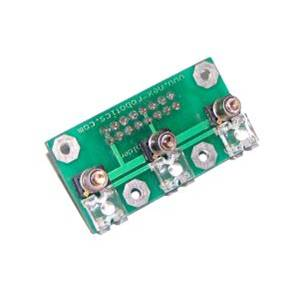
\includegraphics[width=0.8\linewidth]{line_sensor}
		\vfill
			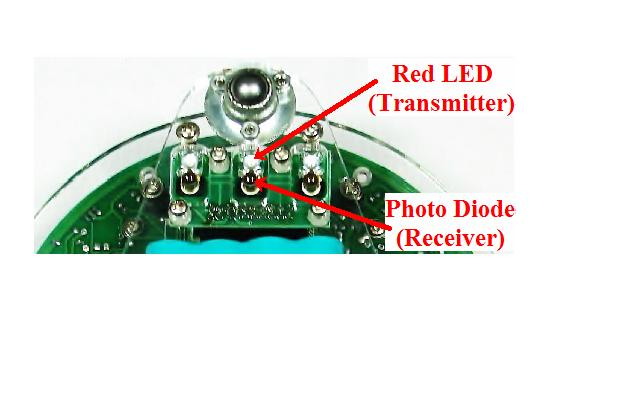
\includegraphics[width=\linewidth]{line_sensor_on_fb}
		\end{minipage}	
\end{frame}	

%Slide-13 Position Encoder
\begin{frame}
	\frametitle{Sensors on Firebird V Platform (cont.)} 
	4. Position Encoder	\pause
		\vfill
		\begin{minipage}[c]{0.5\textwidth}
			\begin{enumerate}
				\item <+-|alert@+> Transmitter: IR Transmitter  \qquad Receiver: PhotoTransistor \\[10pt]
				\item <+-|alert@+> Count on Firebird: 02 \\[10pt]
			\end{enumerate}
		\end{minipage}
	%	\pause
		\hfill
		\begin{minipage}[c]{0.4\textwidth}
			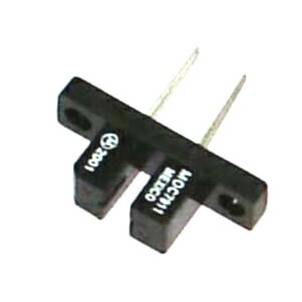
\includegraphics[width=0.6\linewidth]{Position_encoder}
		\vfill
			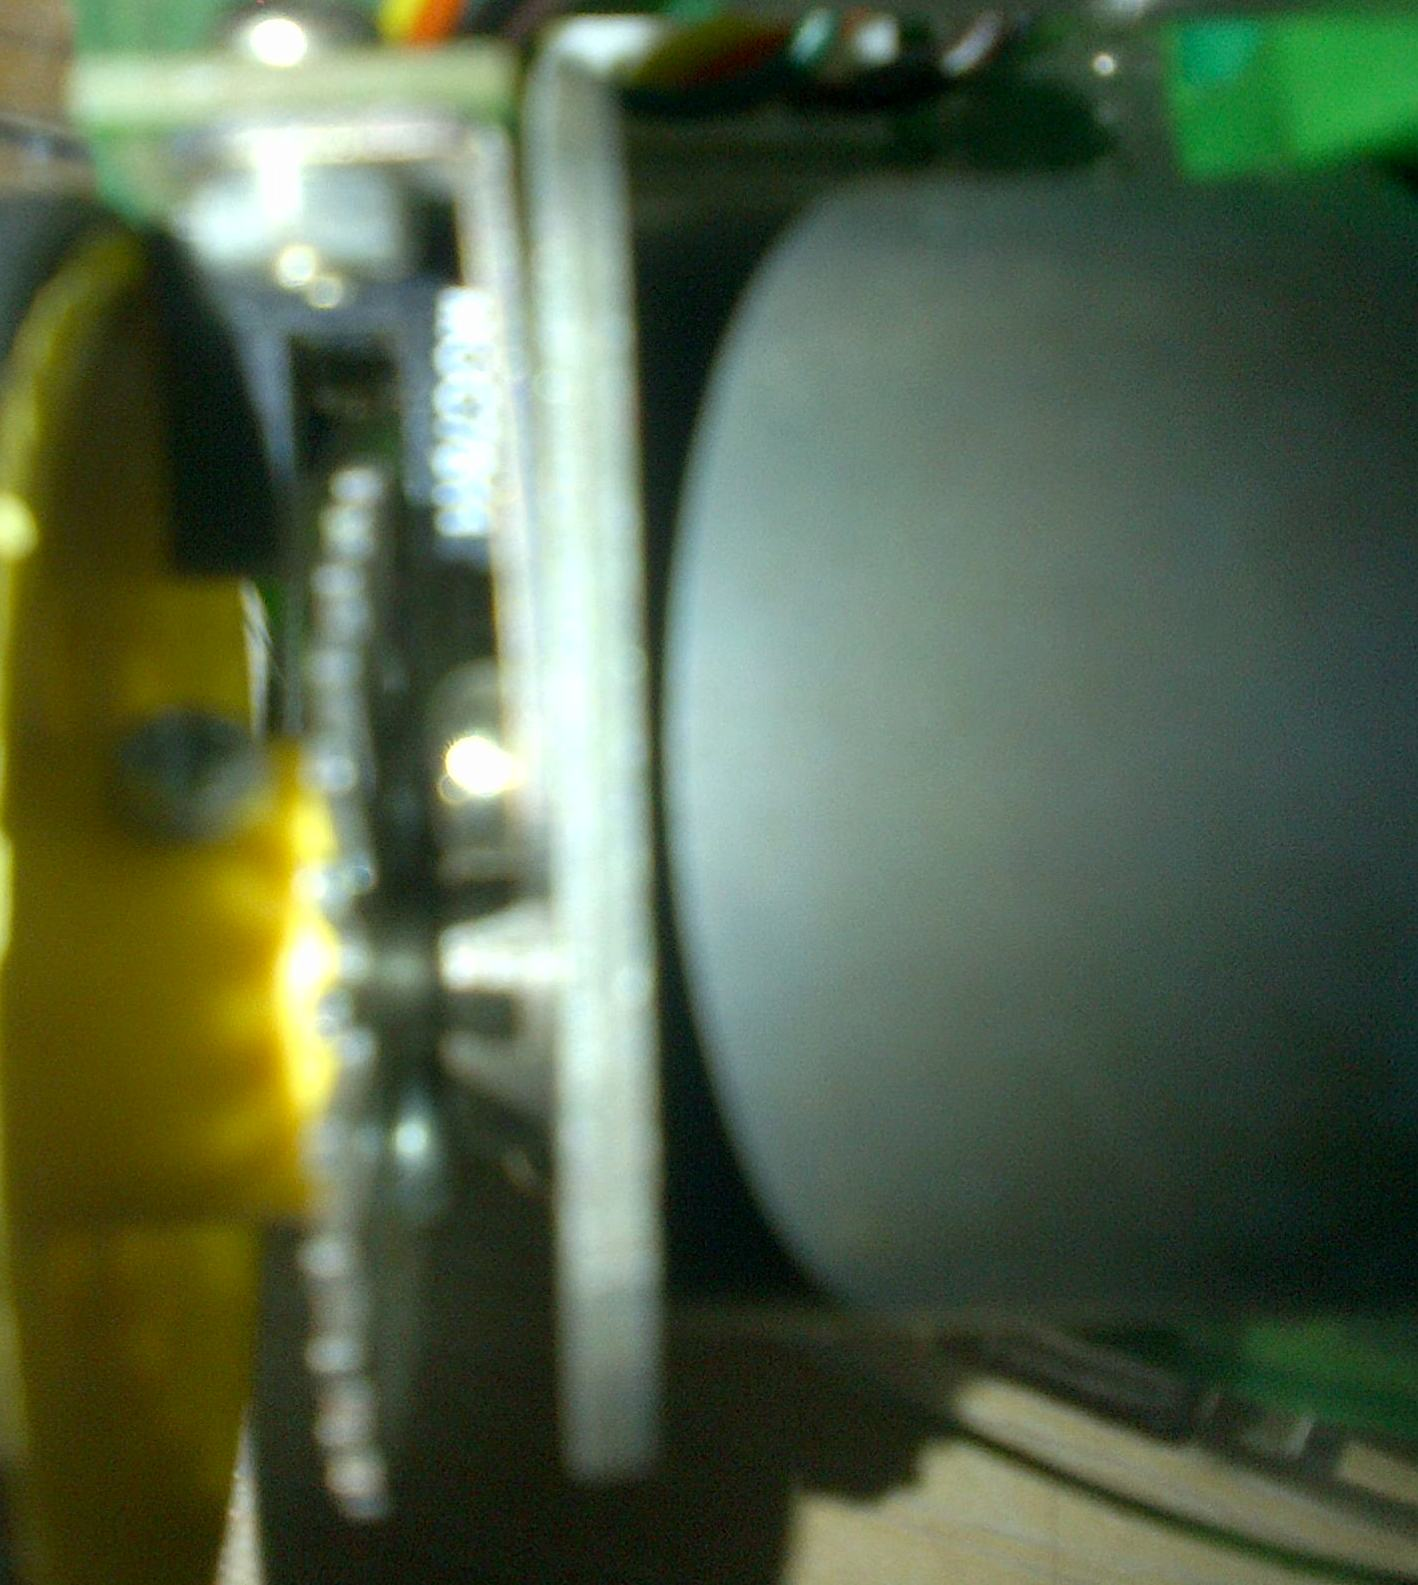
\includegraphics[width=0.6\linewidth]{encoder_on_fb}
		\end{minipage}	
\end{frame}	

%Slide-14 TSOP
\begin{frame}
	\frametitle{Sensors on Firebird V Platform (cont.)} 
	5. Infrared TSOP Receiver	\pause
		\vfill
		\begin{minipage}[c]{0.5\textwidth}
			\begin{enumerate}
				\item <+-|alert@+> Receiver: PhotoTransistor \\[10pt]
				\item <+-|alert@+> TSOP1738 \\[10pt]
				\item <+-|alert@+> Count on Firebird: 01 \\[10pt]
			\end{enumerate}
		\end{minipage}
	%	\pause
		\hfill
		\begin{minipage}[c]{0.4\textwidth}
			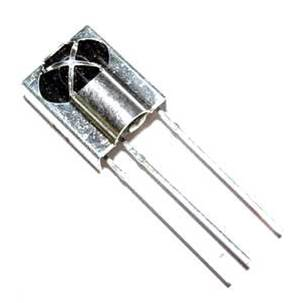
\includegraphics[width=0.6\linewidth]{tsop_receiver} \\[10pt]
		\vfill
			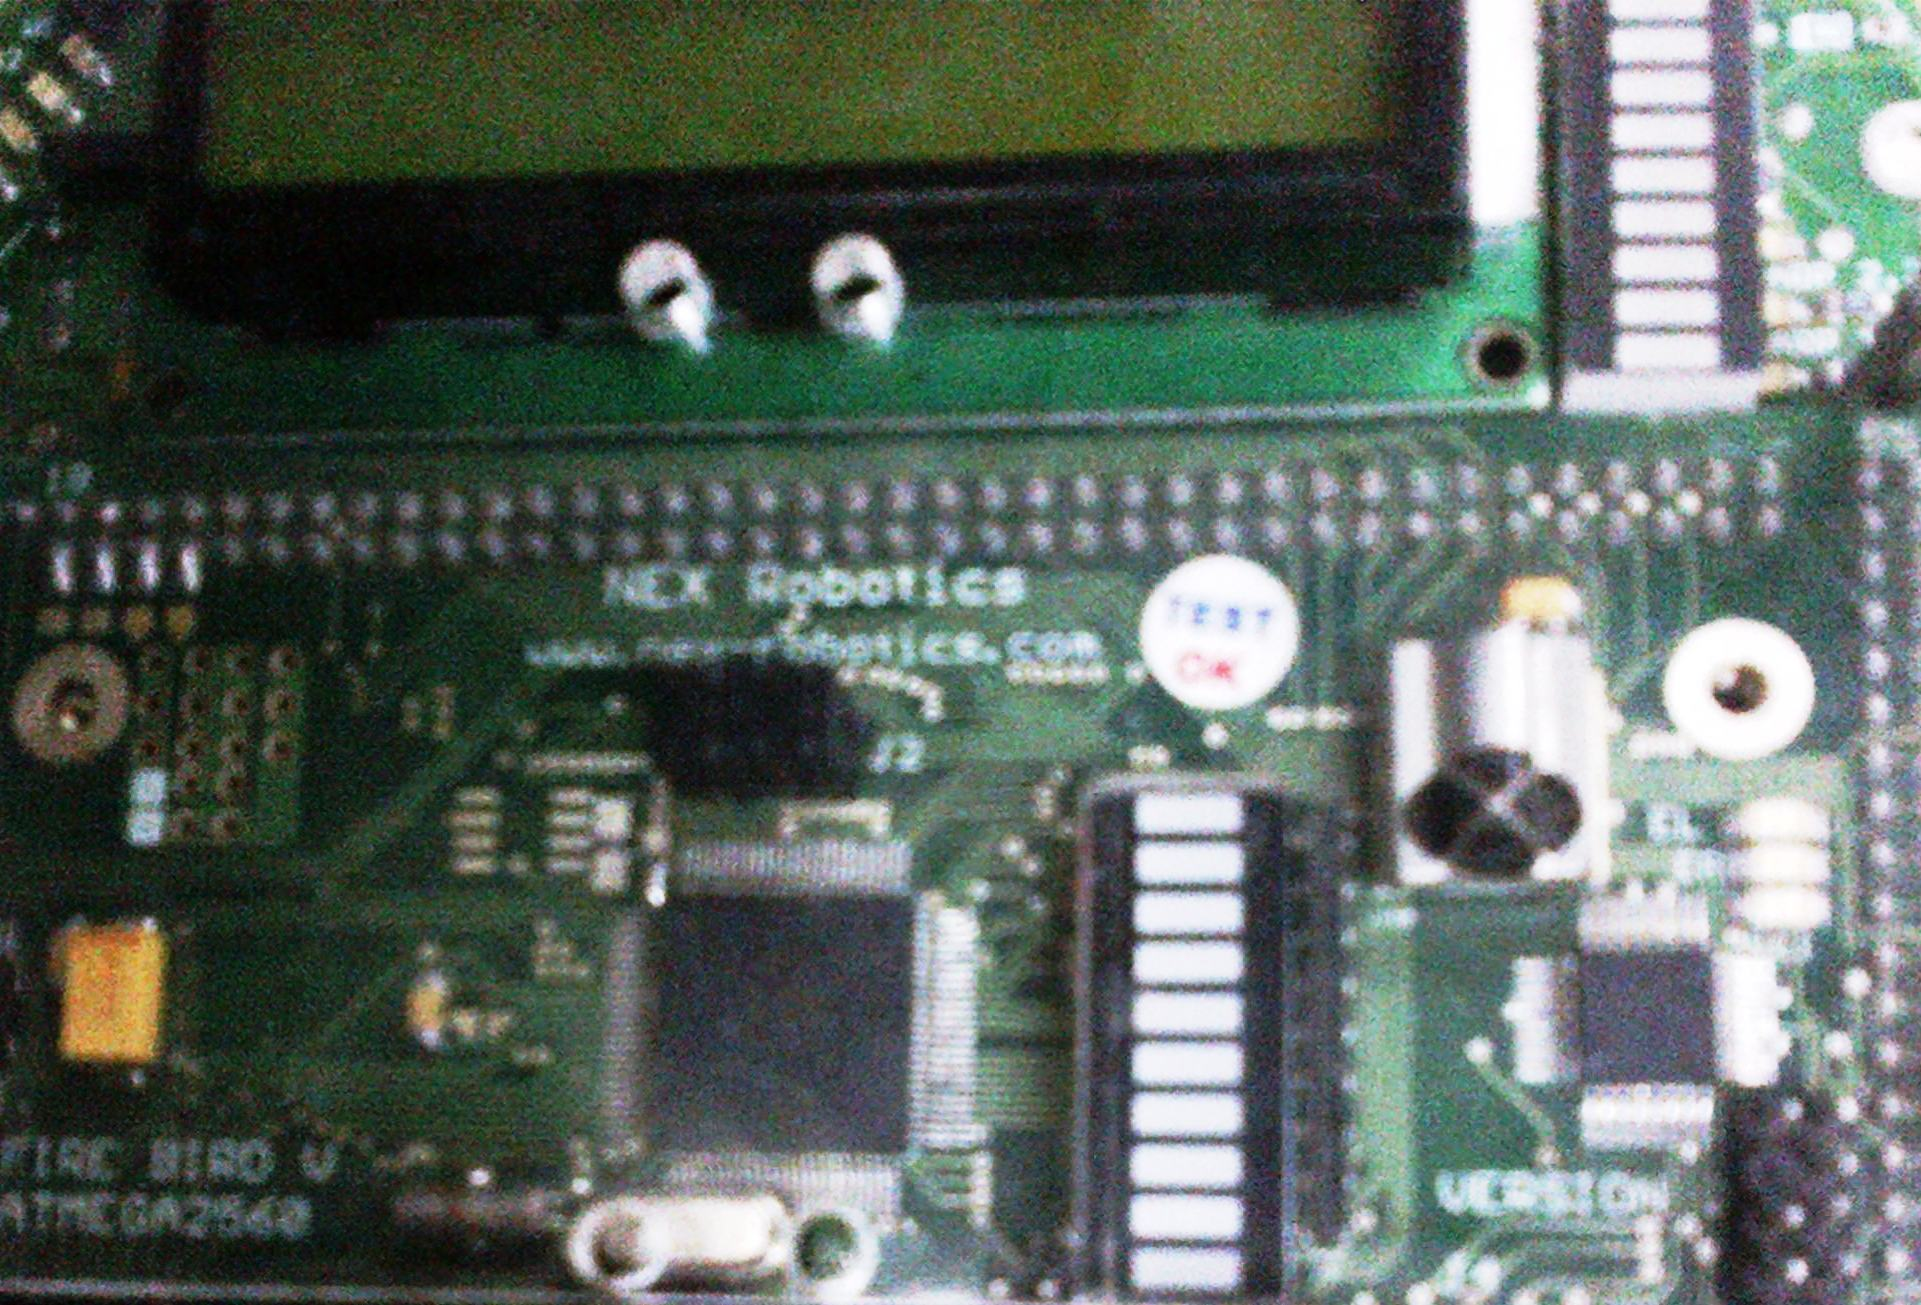
\includegraphics[width=0.6\linewidth]{tsop_on_fb}
		\end{minipage}	
\end{frame}	

%Slide-15 Servo Pod
\begin{frame}
	\frametitle{Sensors on Firebird V Platform (cont.)} 
	6. Servo Mounted Sensor Pod	\pause
		\vfill
		\begin{minipage}[c]{0.5\textwidth}
			\begin{enumerate}
				\item <+-|alert@+> Purpose: Mount Camera or Sensor 
				\item <+-|alert@+> Count on Firebird: Optional Add-on Module
			\end{enumerate}
		\end{minipage}
		%\pause
		\hfill
		\begin{minipage}[c]{0.4\textwidth}
			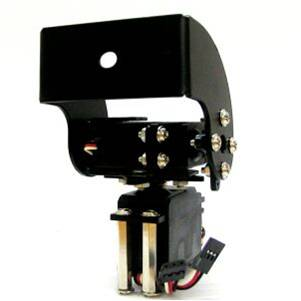
\includegraphics[width=\linewidth]{servo_pod}
		\end{minipage}	
\end{frame}		

%Slide-16 Accelerometer
\begin{frame}
	\frametitle{Sensors on Firebird V Platform (cont.)} 
	7. Accelerometer	\pause
		\vfill
		\begin{minipage}[c]{0.5\textwidth}
			\begin{enumerate}
				\item <+-|alert@+> Accelerometer is used for measuring acceleration in particular direction \\[10pt]
				\item <+-|alert@+> Count on Firebird: Optional Add-on Module
			\end{enumerate}
		\end{minipage}
	%	\pause
		\hfill
		\begin{minipage}[c]{0.4\textwidth}
			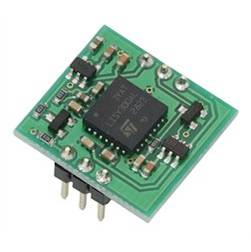
\includegraphics[width=\linewidth]{accelerometer}
		\end{minipage}	
\end{frame}	

%Slide-17 Gyroscope
\begin{frame}
	\frametitle{Sensors on Firebird V Platform (cont.)} 
	8. Gyroscope	\pause
		\vfill
		\begin{minipage}[c]{0.5\textwidth}
			\begin{enumerate}
				\item <+-|alert@+> Gyroscope are devices used for providing stability and maintain fixed orientation \\[10pt]
				\item <+-|alert@+> Count on Firebird: Optional Add-on Module
			\end{enumerate}
		\end{minipage}
		%\pause
		\hfill
		\begin{minipage}[c]{0.4\textwidth}
			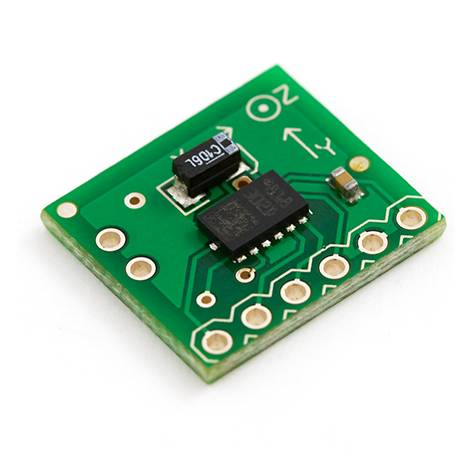
\includegraphics[width=\linewidth]{gyroscope}
		\end{minipage}	
\end{frame}	

%Slide-18 Ultrasonic
\begin{frame}
	\frametitle{Sensors on Firebird V Platform (cont.)} 
	9. Ultrasonic Sensor	\pause
		\vfill
		\begin{minipage}[c]{0.5\textwidth}
			\begin{enumerate}
				\item <+-|alert@+> Ultrasonic sensor is used for object detection \\[10pt]
				\item <+-|alert@+> Count on Firebird: Optional Add-on Module
			\end{enumerate}
		\end{minipage}
	%	\pause
		\hfill
		\begin{minipage}[c]{0.4\textwidth}
			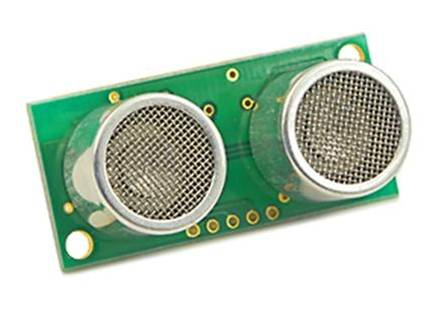
\includegraphics[width=\linewidth]{ultrasonic}
		\end{minipage}	
\end{frame}

%Slide-19 PIR-Motion Sensor
\begin{frame}
	\frametitle{Sensors on Firebird V Platform (cont.)} 
	10. Motion Sensor	\pause
		\vfill
		\begin{minipage}[c]{0.5\textwidth}
			\begin{enumerate}
				\item <+-|alert@+> PIR Motion Sensor is used for detecting motion of live object. \\[10pt]
				\item <+-|alert@+> Count on Firebird: Optional Add-on Module
			\end{enumerate}
		\end{minipage}
	%	\pause
		\hfill
		\begin{minipage}[c]{0.4\textwidth}
			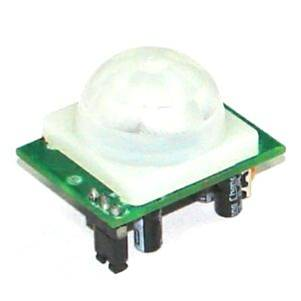
\includegraphics[width=\linewidth]{PIR_motion}
		\end{minipage}	
\end{frame}

%Slide-20 GPS
\begin{frame}
	\frametitle{Sensors on Firebird V Platform (cont.)} \pause
	11. Global Positioning System(GPS)	
		\vfill
		\begin{minipage}[c]{0.5\textwidth}
			\begin{enumerate}
				\item <+-|alert@+> GPS module are devices which receives GPS signal to locate itself on earth  \\[10pt]
				\item <+-|alert@+> GPS module gives latitude and longitude information  \\[10pt]
				\item <+-|alert@+> Count on Firebird: Optional Add-on Module
			\end{enumerate}
		\end{minipage}
	%	\pause
		\hfill
		\begin{minipage}[c]{0.4\textwidth}
			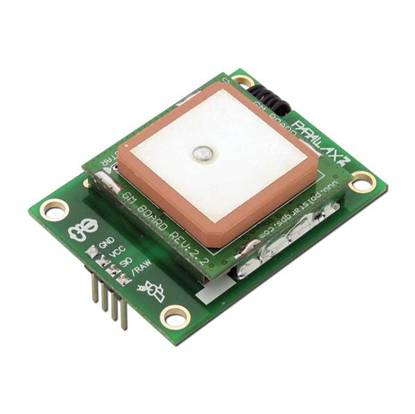
\includegraphics[width=\linewidth]{GPS}
		\end{minipage}	
\end{frame}

%******** End of subsection-2 (Senosr)*************

%******** Start of subsection-3 (Actuator)*************
\subsection{Actuators}
%Slide-21 Motors
\begin{frame}
	\frametitle{Actuators} \pause
		\begin{enumerate}
			\item<1->	Two 60 RPM DC Geared Motor \\[8pt] 
			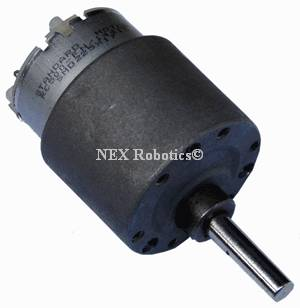
\includegraphics[width=0.15\linewidth]{dc_motor} \\[10pt]
			\item<2->	Servo Motors\\[8pt]
			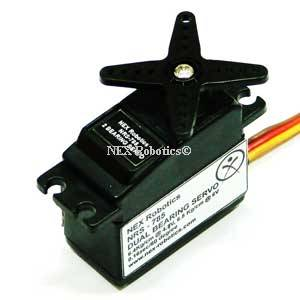
\includegraphics[width=0.15\linewidth]{servo} \hspace{2cm}
		\end{enumerate}
\end{frame}

%******** End of subsection-3 (Actuator)*************

%******** Start of subsection-4 (Control)*************
\subsection{Control}
%Slide-22 Control
\begin{frame}
	\frametitle{Control Room of Robot} \pause
		\begin{enumerate}
			\item<1->	NXP Phillips Manufactured ARM-7 architecture based LPC2148 microcontroller 
		\end{enumerate}
\end{frame}

%******** End of subsection-4 (Control)*************

%******** Start of subsection-5 (Intelligence)*************
\subsection{Intelligence}
%Slide-23 Intelligence
\begin{frame}
	\frametitle{How is Robot Made Intelligent} \pause
		\begin{enumerate}
			\item<1->	Language used for programming: EMBEDDED 'C'
			\item<2->	EMBEDDED 'C' similar to C.  
		\end{enumerate}
\end{frame}

%******** End of subsection-5 (Intelligence)*************

%******** Start of subsection-6 (Power)*************
\subsection{Power}
%Slide-24 Power
\begin{frame}
	\frametitle{Powering the Robot} \pause
		\begin{enumerate}
			\item<1->	Battery Powered:	9.6V, 2100mAH, NiMH battery \\[8pt] 
			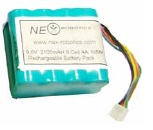
\includegraphics[width=0.15\linewidth]{battery} \\[10pt]
			\item<2->	Auxillary Power:  9V, 1A Adaptor \\[8pt]
			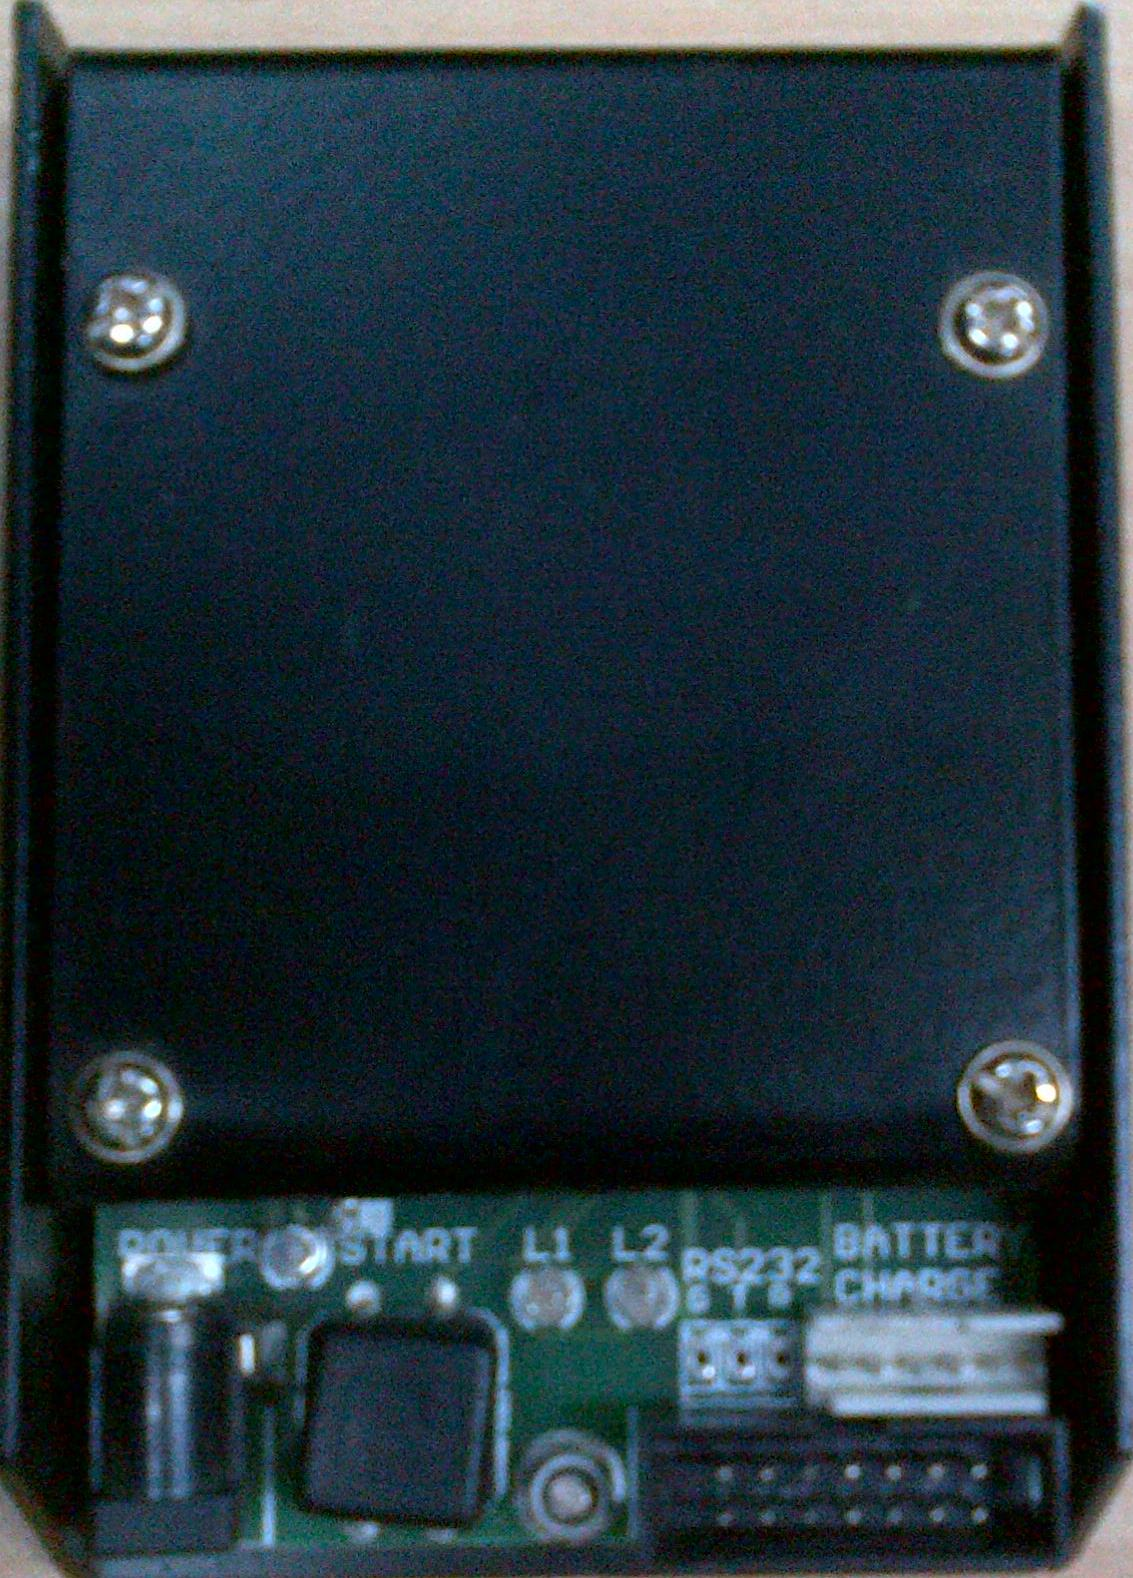
\includegraphics[width=0.15\linewidth]{auxillary} \\[10pt]  
		\end{enumerate}
\end{frame}

%******** End of subsection-6 (Power)*************

%******** Start of subsection-7 (Communication)*************
\subsection{Communication}
%Slide-25 Communication
\begin{frame}[shrink=5]
	\frametitle{Communication} \pause
		
		\begin{minipage}[c]{\textwidth}
			\begin{enumerate}[$\checkmark$]
				\item<1->	Wired Communication: Between Robot and System \pause \\
				\item<1->	USB; RS-232 Serial; USB-to Serial \\
				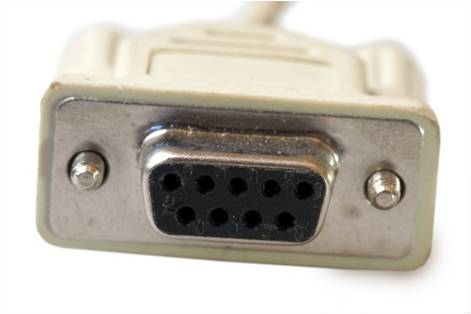
\includegraphics[width=0.15\linewidth]{rs232} \hspace{2cm}
				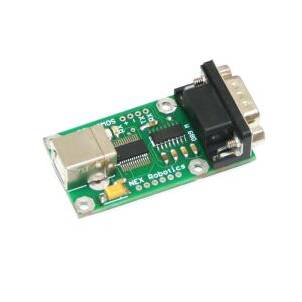
\includegraphics[width=0.15\linewidth]{usbtoserial} \\
			\end{enumerate}
		\end{minipage}
		
		\pause
		\vfill
				\begin{minipage}[c]{\textwidth}
			  \begin{enumerate}[$\checkmark$]
				\item<2->	Wire-less Communication:Between Robot and System and Robot and Robot \pause \\
			  \item<2->	X-bee based on IEEE 802.15.4 Protocol\\
				\includegraphics[width=0.1\linewidth]{xbee}\\ \pause
				\item<3->	Infrared Remote\\
				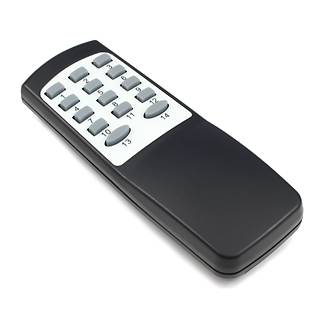
\includegraphics[width=0.1\linewidth]{tv_remote}\\
			\end{enumerate}
		\end{minipage}
\end{frame}

%******** End of subsection-7 (Communication)*************

%******** Start of subsection-8 (Indicating Devices)*************
\subsection{Indicating Devices}
%Slide-26 Indicating Devices
\begin{frame}
	\frametitle{Indicating Devices} \pause
		\begin{minipage}[c]{0.5\textwidth}
			\begin{enumerate}[$\checkmark$]
				\item<1->	16x2 Alpha numeric LCD \pause \\[2pt]
				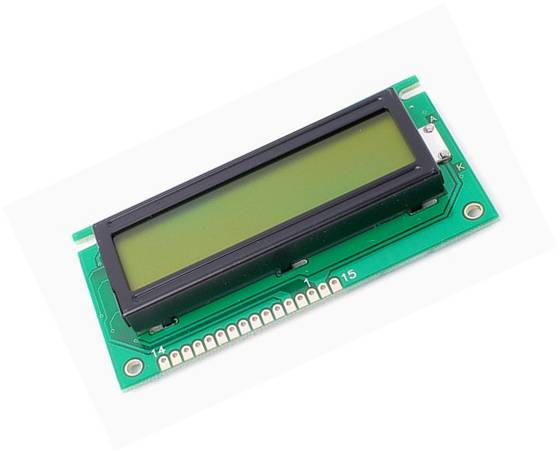
\includegraphics[width=0.4\linewidth]{lcd} \\
			\end{enumerate}
		\end{minipage}
		
		\pause
		\vfill
				\begin{minipage}[c]{0.5\textwidth}
			\begin{enumerate}[$\checkmark$]
				\item<2->	Buzzer \pause \\[2pt]
				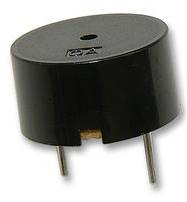
\includegraphics[width=0.2\linewidth]{buzzer}\\
			\end{enumerate}
		\end{minipage}
		
		\pause
		\vfill
		\begin{minipage}[c]{0.5\textwidth}
			\begin{enumerate}[$\checkmark$]
				\item<3->	Bar-LED \pause \\[2pt]
				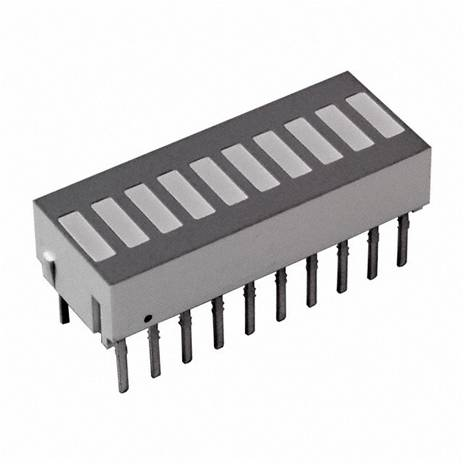
\includegraphics[width=0.3\linewidth]{barled}\\
			\end{enumerate}
		\end{minipage}
		
		
\end{frame}
%******** End of subsection-8 (Indicating Devices)*************

%******** Start of subsection-9 (Block Diagram)*************
\subsection{Block Diagram}
%Slide-27 Block Dig.
\begin{frame}
	\frametitle{Block Diagram of LPC2148 ARM7 based Robot} \pause
		%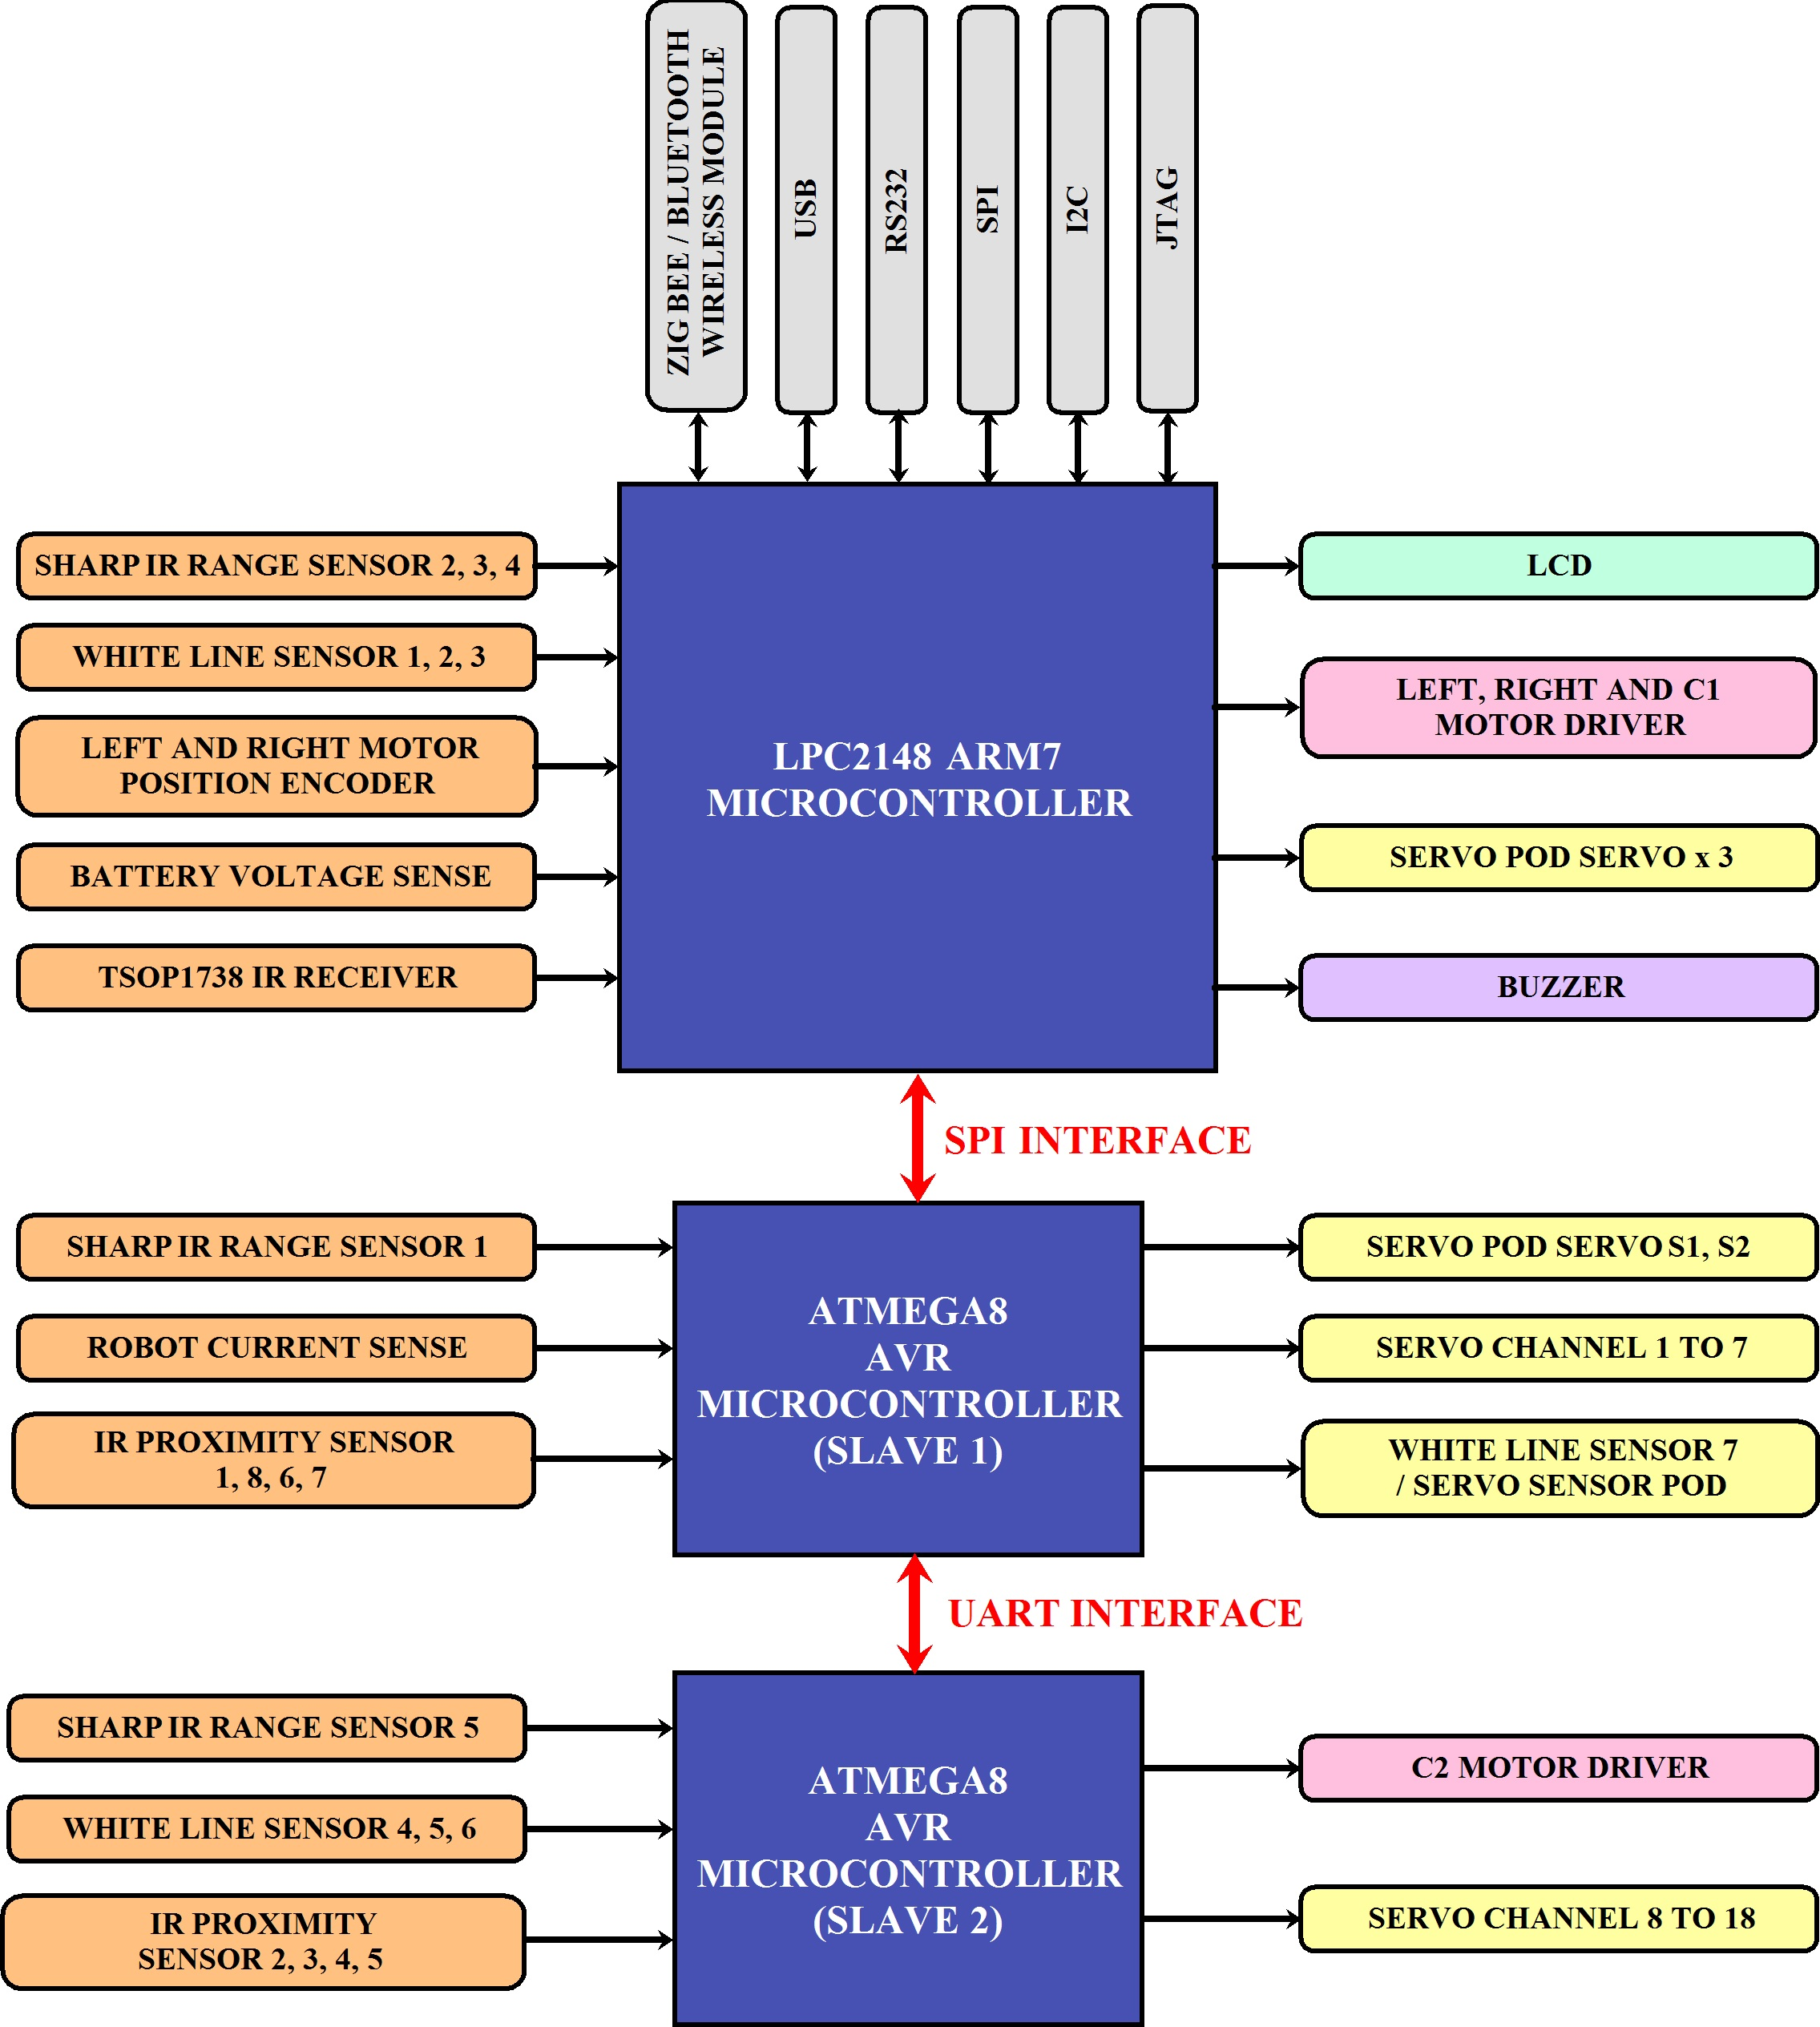
\includegraphics[width=\linewidth]{block_diagram}
		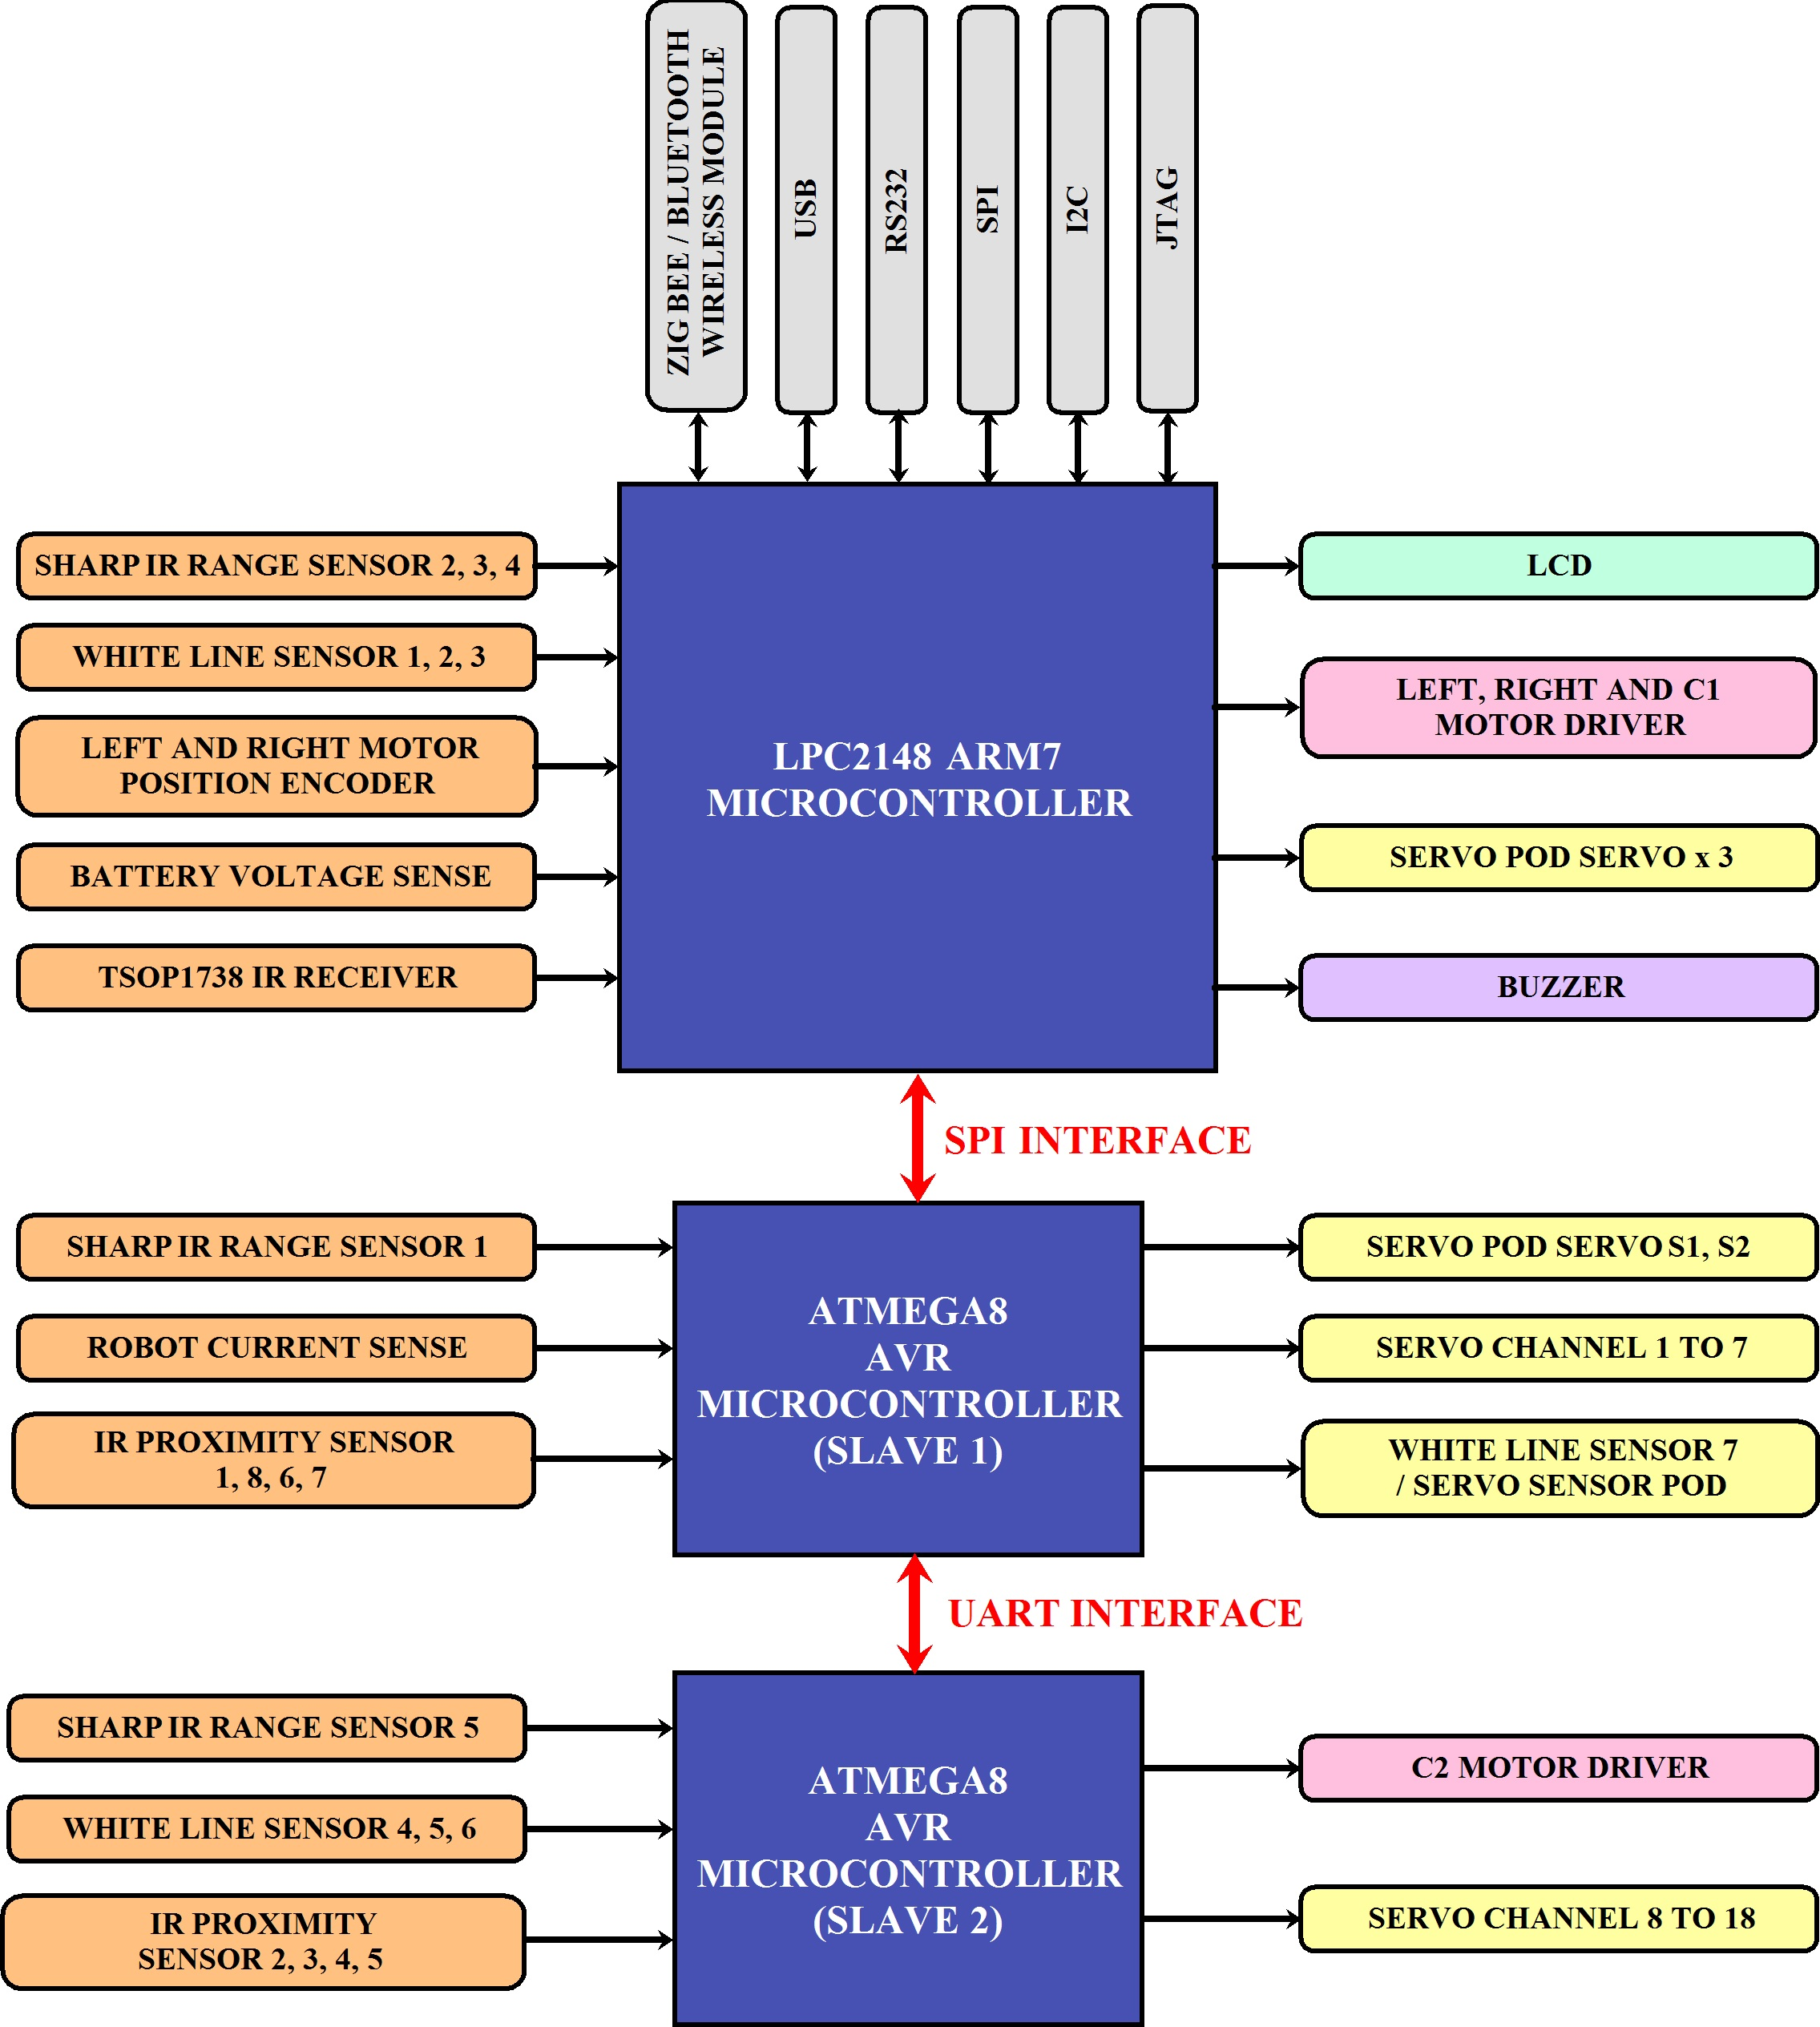
\includegraphics[scale=0.1]{block_diagram}
\end{frame}

%******** End of subsection-9 (Block Diagram)*************

\begin{frame}
\hskip4cm
\textbf{\LARGE Thank You!} \\[20pt]
\hskip3cm
\scriptsize Post your queries on: 
\hyperref[www.e-yantra.org]{\color{blue} http://qa.e-yantra.org/ \color{black}} 
\end{frame}
\end{document}

